\documentclass[14pt,a4paper]{article}
\usepackage{txfonts}
\usepackage{url}
\usepackage[colorlinks, citecolor=blue, urlcolor=blue]{hyperref}
\usepackage[utf8]{inputenc}
\usepackage[spanish]{babel}
\usepackage{amsmath}
\usepackage{amsfonts}
\usepackage{amssymb}
\usepackage{makeidx}
\usepackage{graphicx}
\usepackage{lmodern}
\usepackage{kpfonts}
\usepackage{fourier}
\usepackage[left=2cm,right=2cm,top=2cm,bottom=2cm]{geometry}
\author{Rodriguez Lopez Francisco Javier}


\begin{document}
\begin{center}
\paragraph{\large UNIVERSIDAD POLITECNICA DE LA ZONA METROPOLITANA DE GUADALAJARA}


\includegraphics[scale=1]{Upzmg.png} 
\end{center}
\begin{center}
\textbf{\LARGE Avance 1}\\
\end{center}
\begin{center}
\textbf{\LARGE Brazo Robotico}
\end{center}


\large{Integrantes:}\\
\large{Guzman Vazquez Jaime Alan.\\
Perez de Alba Santiago Eduardo.\\
Romero Jauregui Osvaldo.\\
Cabrera Gutierrez Raul.\\
Gutierrez Olivares Rogelio.\\
Rodriguez Lopez Francisco Javier.\\

Fecha: 20 de septiembre del 2019.\\

Curso: Sep-Dic 2019.\\

Docente: Moran Garabito Carlos Enrique.\\}

\newpage

\section{Objetivo General:}

Creacion de un brazo robòtico con la finalidad de adaptacion a tareas complejas que el personal humano no realice con exactitud, mediante los conocimientos adquiridos y la demostracion de habilidades y aptitudes que se tengan.

\section{Justificacion:}

El brazo robotico, es una herramienta eficiente para ambientes, insutria-empresariales, para funcion y mejora del trabajo del personal comun, que mejora la rapidez, fluidez y sustencion del trabajo a realizar, o en este caso alguna tarea en particular. El brazo robotico suplementa en eficiencia las tareas del humano, al fin de remplazar la lentitud y errores que este tiene.\\
El proyecto planteado en sintesis, tiene como idea, el  poder suplementar esas tareas empresariales que cuesta mucho dinero, energia y trabajo en cuestion, tratando complejos casos como la falta de personal, siendo este la sustitucion perfecta para las manos laborales ordinarias, ambientado en el sector de automatizacion, y robotica, el cual pueda tambien agarrar temas, de control, y sustentacion de las herramientas que se utilizaran en este proyecto, que en relevancia nos deje tanto a nosotros como conocimiento, a la sociedad uan herramienta que pueda ser mejor innovada y utilizada, en otros campos, no simplemente industriales.\\
Estructurado en primera instancia a la industria, la mecatronica y sus amplias gamas de estudio que puede cubrir para la mejoracion e implentacion, en las tareas que este pueda realizar, siendo varias y de ello, poder visulalizar en que constancia este dispositivo este apto para temas de mayor complejidad, viendo las problematicas que este tiene, a la  hora de implementarlos el sector de automatizacion, y las ganancias mismas de este.

\section{Marco Teorico:}

Robot:
Se suele entender también que un robot goza de un elevado grado de autonomía y de autoplanificación, de modo que es capaz de hacer su tarea sin intervención del operador, tomando las decisiones oportunas a partir de la información que recaban sus sensores, gracias al programa almacenado en su memoria.
Brazo:\\
Extremidad superior del cuerpo humano, que va desde el hombro hasta el final de la mano.\\

Brazo Robotico:
La definición adoptada por el Instituto Norteamericano de Robótica aceptada internacionalmente para Robot es:\\

“Manipulador multifuncional y reprogramable, diseñado para mover materiales, piezas, herramientas o dispositivos especiales, mediante movimientos programados y variables que permiten llevar a cabo diversas tareas”.\\
Un robot industrial son una serie de artilugios mecánicos y electrónicos destinados a realizar de forma automática y sin necesidad de intervención humana. determinados procesos de fabricación o manipulación.\\
Por lo tanto, Robótica será:  Una rama de la Inteligencia Artificial que se ocupa de las máquinas inteligentes.
\newpage
\section{Cronograma de Trabajo:}
Cronograma de trabajo, fechas establecidas del 12 de  Septiembre del 2019 al dia de entrega, 18 de mayo del 2020

\begin{center}
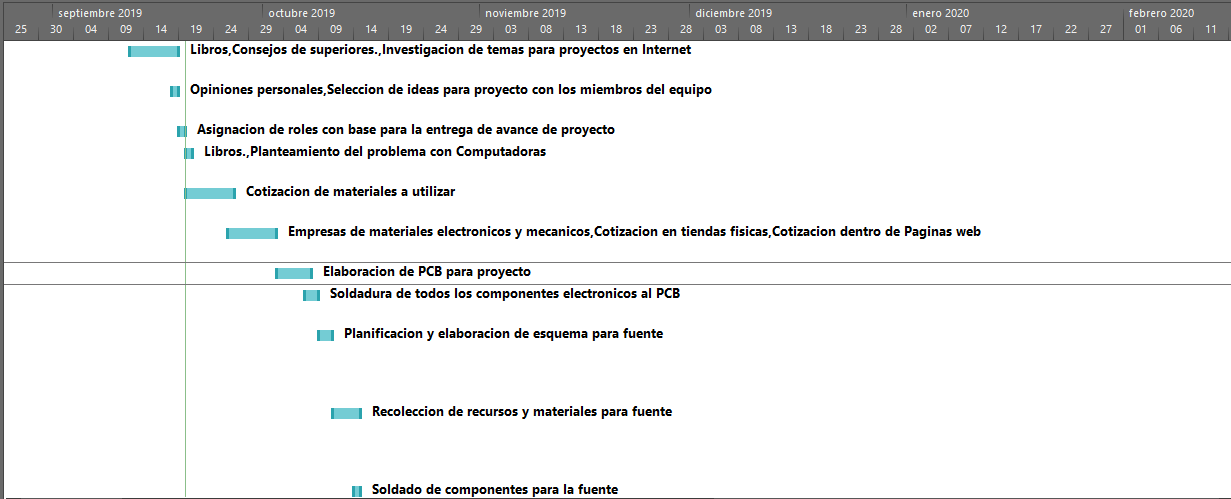
\includegraphics[width=17cm]{CronogramaTrabajo/1.png}\\

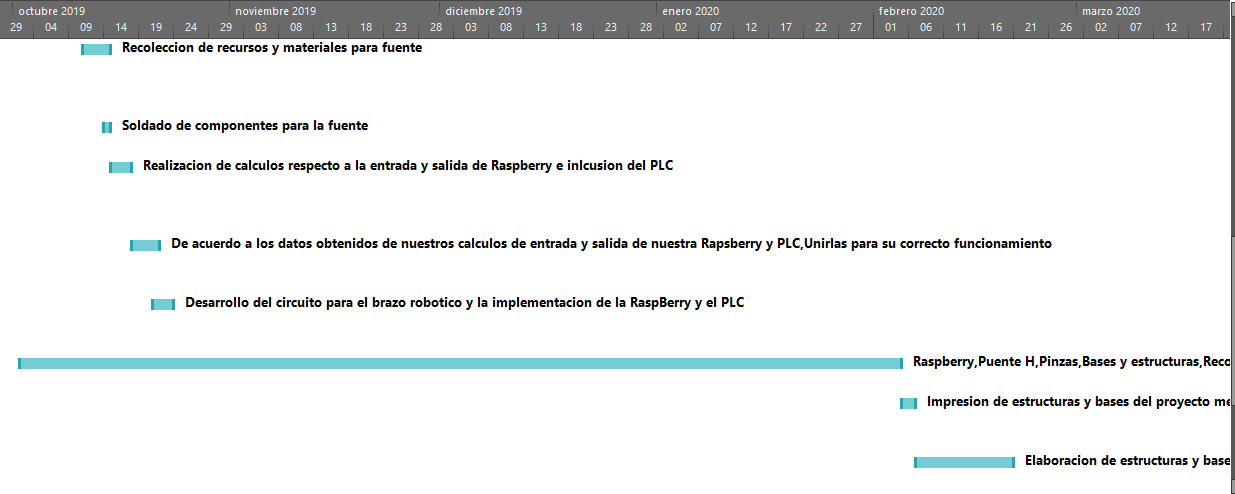
\includegraphics[width=17cm]{CronogramaTrabajo/2.png}\\

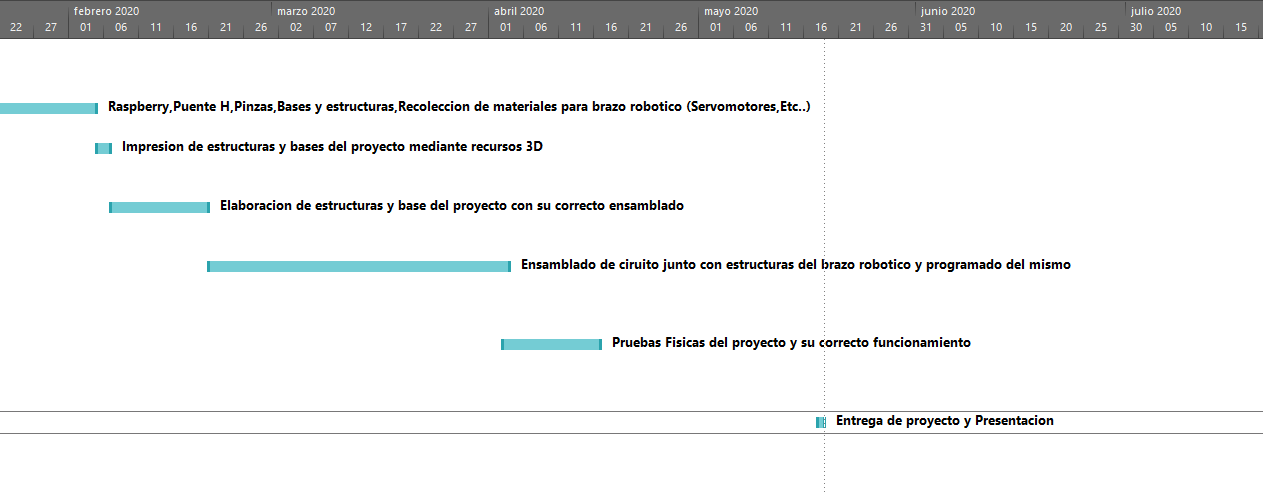
\includegraphics[width=17cm]{CronogramaTrabajo/3.png}  
\end{center}
\newpage
\section{Definicion de Tareas:}
Aqui se establece, cada parte de la realizacion de este proyecto, desde la planeacion del dispositivo, hasta el motaje en fisico de este.

\begin{center}
 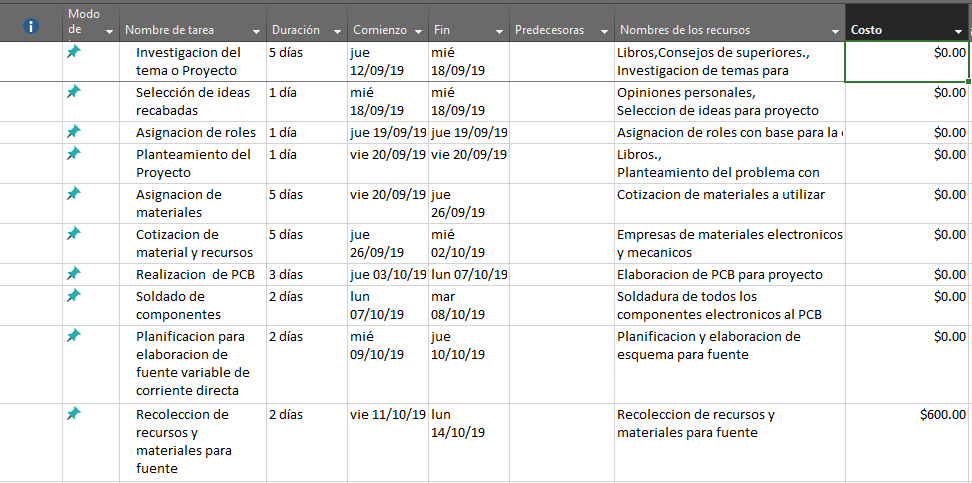
\includegraphics[width=15cm]{DefinicionTareas/4.png}\\
 
 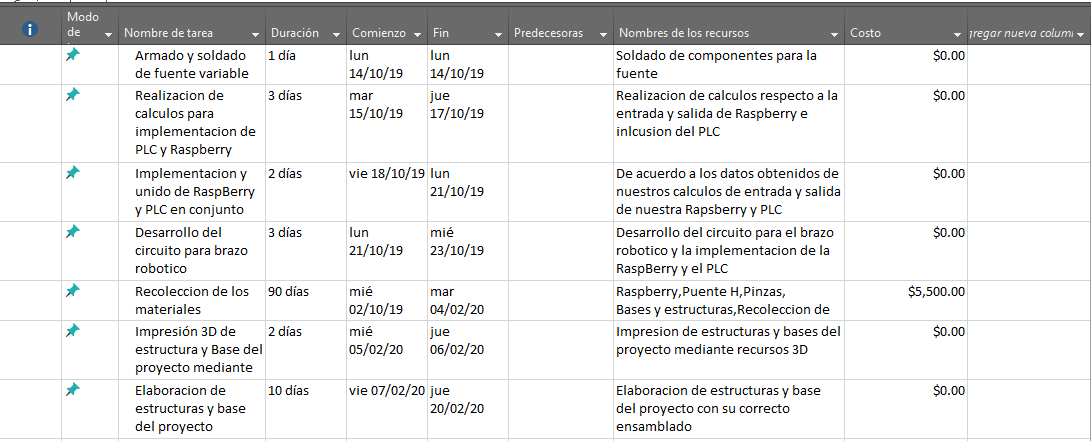
\includegraphics[width=15cm]{DefinicionTareas/5.png}\\
 
 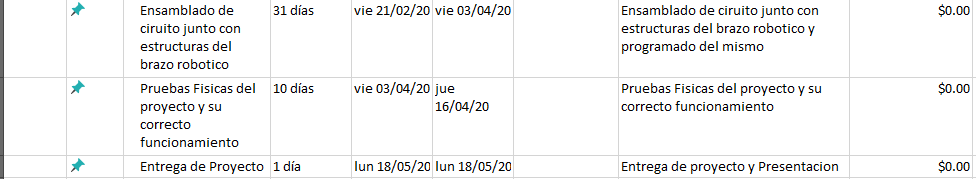
\includegraphics[width=15cm]{DefinicionTareas/6.png} 
\end{center}
\newpage
\section{Primer Bosquejo:}
Se ve una previsualizacion, de como quedaria establecido el proyecto a final de entrega, con algunos detallles extras que se puedan agregar en un futuro, para la mejor estetica de este.

\begin{center}
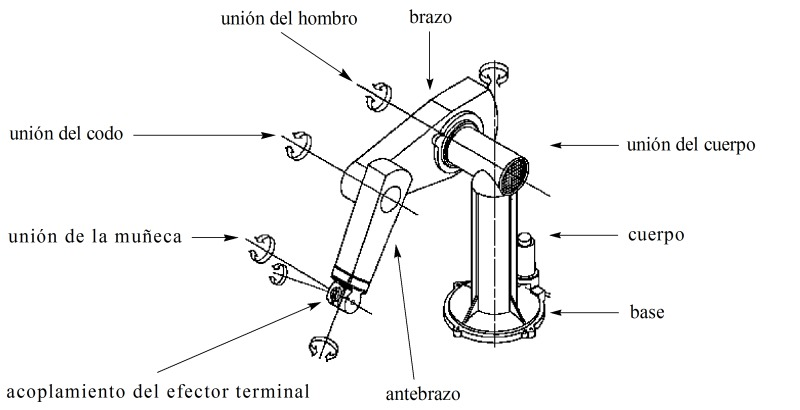
\includegraphics[width=10cm]{Bosquejo.jpeg} 
\end{center}

\section{Propuesta de Materiales:}

\subsection{Elementos consturctivos}
Manipulador o brazo mecanico.\\
Elementos motrices o actuadores.\\
Controlador.\\
Efector terminal.\\
Sensores de informacion.

\subsection{Manipulador}
Es el conjunto de elementos mecanicos que permiten el movimiento del efector termina. En la estructura interna del manipulador se encuentran ubicador muchas veces los elementos motrices, engranajes y tranmisiones que soportan el movimiento de las cuatro partes, que por lo geneal conforman el manipulador, las cuales son:\\
1-Base o pedestal de fijacion.\\
2-Cuerpo.\\
3-Brazo.\\
4-Antebrazo.\\
\subsection{Elementos motrices o Actuadores}
\paragraph{Neumaticos}
Emplean aire comprimido como fuente de energia y son adecuados en el control de movimientos rapidos, pero su precision es limitada.
\paragraph{Hidraulicos}
Los actuadores hidraulicos son recomendables en los manipuladores que tiene una gran capacidad de carga, junto a una precisa regulacion de velocidad.
\paragraph{Electricos}
Los motores electricos son los mas utilizados, gracias a su precision y la facilidad de control.
\subsection{Controlador}
Es el dispositivo encargado de regular el movimiento de todos los elementos del manipulador, y de realizar los calculos y procesado de la informacion. La complejidad del control varia segun los pramatros que se gobiernan.
\subsection{Efector Terminal}
Es la garra o herramienta que se le acopla a la muneca del manipulador, siendo el encargado de materializar el trabajo previsto por ejemplo, este puede ser una tenaza, un electroiman, o algun otro aparato. En general, y de acuerdo al tipo de aplicacion, la problematica del efector terminal radica en que este ha de posser una elevada capacidad de carga y al mismo tiempo es importante que tenga un peso y tamano reducido. Por esto, en muchas ocasiones es necesario disenar el efector terminal de acuerdo a los requerimientos de la aplicacion en que se utilizara.
\subsection{Sensores de Informacion}
Los robot inteligentes son aquellos capaces e adaptarse al ambiente y tomar decisiones en tiempo real, adecuadas para situacion. La informacion que ellos reciben les hace autoprogramables, es decir,alteran su actuar en funcion de la situacion externa, lo que los hace poseer un cierto grado de inteligencia artificial. A este respecto, las informaciones mas solicitadas por los robots son las que hacen referencia a la posicion, velocidad, aceleracion, fuerzas,pares, dimensiones y contornos de objetos, y temperatura.

\section{Presupuesto:}

\begin{tabular}{|l|l|l|l|}
\hline
	Producto & Piezas & Precio & Total\\
\hline
	Impresion 3D & 5 & 70 & 350\\

\hline
	Capacitores 33pF & 2 & 5 & 10\\
\hline
	 Circuitos integrados L293B & 2 & 15 & 30\\
\hline
	Resistencias varias & 20 & 2 & 40\\
\hline
	Diodos1N4004G & 16 & 5 & 80\\
\hline
	1 Switch & 1 & 10 & 10\\

\hline
	Fuente CA-CD & 1 & 600 & 600\\
\hline
	Push bottons & 8 & 2 & 16\\
\hline
cautin & 1 & 150 & 150\\
\hline
	Estaño & 1 & 30 & 30\\
\hline
	Multimetro & 1 & 100 & 100\\
\hline
Motores DC & 5 & 400 & 2000\\
\hline
\end{tabular}

\section{Referencias:}
\url{www.grupoisis.uma.es/microbot/public/robots.pdf}\\

\url{http://repositorio.usfq.edu.ec/bitstream/23000/3840/1/112562.pdf}\\

\url{https://electrosite01.wordpress.com/2014/06/04/proyecto-brazo-robotico-compra-de-materiales/}\\

\url{https://www.feriadelasciencias.unam.mx/anteriores/feria21/feria361_01_desarrollo_de_brazo_robotico_para_multiples_aplica.pdf}
\end{document}